\documentclass{book}

\usepackage[utf8]{inputenc}
\usepackage{titlesec}
\usepackage{easylist}
\usepackage{hanging}
\usepackage{hyperref}
\usepackage[a4paper,top=2.0cm,bottom=2.0cm,left=2.0cm,right=3.0cm]{geometry}
\usepackage{blindtext}
\usepackage{tipa}
\usepackage{epigraph}
\usepackage{enumerate}
\usepackage{longtable}
\usepackage{setspace}
\usepackage{verbatim}
\usepackage[T1]{fontenc}
\usepackage{graphicx}
\usepackage[italian]{babel}
\usepackage{amsmath}
\usepackage{pbox}
\usepackage{fancyhdr}
\usepackage{cancel}
\usepackage{tabularx}
\usepackage{booktabs}
\usepackage{multirow}
\usepackage{longtable}
\usepackage{tikz}
\usepackage{tikz-qtree}
\usepackage{subfig}
\usepackage{xcolor}
\usepackage{amssymb}
\usepackage{amsmath}
\usepackage{mathrsfs}
\usepackage{textcomp}
\usepackage{circuitikz}
\usepackage{pifont}
\usepackage{imakeidx}
\usepackage{verbatim}
\usepackage{dsfont}
\usepackage{listings}
\usepackage{color}
\usepackage{upgreek}
\usepackage{tasks}
\usepackage{exsheets}
\usepackage{pgfplots}
\usepackage{lipsum}
\usepackage{array} 
\usepackage{booktabs}

\SetupExSheets[question]{type=exam}

\definecolor{mygreen}{rgb}{0,0.6,0}
\definecolor{mygray}{rgb}{0.5,0.5,0.5}
\definecolor{mymauve}{rgb}{0.58,0,0.82}

\lstset{
  backgroundcolor=\color{white},   % choose the background color; you must add \usepackage{color} or \usepackage{xcolor}; should come as last argument
  basicstyle=\footnotesize,        % the size of the fonts that are used for the code
  breakatwhitespace=false,         % sets if automatic breaks should only happen at whitespace
  breaklines=true,                 % sets automatic line breaking
  captionpos=b,                    % sets the caption-position to bottom
  commentstyle=\color{mygreen},    % comment style
  deletekeywords={...},            % if you want to delete keywords from the given language
  escapeinside={\%*}{*)},          % if you want to add LaTeX within your code
  extendedchars=true,              % lets you use non-ASCII characters; for 8-bits encodings only, does not work with UTF-8
  firstnumber=1000,                % start line enumeration with line 1000
  frame=single,	                   % adds a frame around the code
  keepspaces=true,                 % keeps spaces in text, useful for keeping indentation of code (possibly needs columns=flexible)
  keywordstyle=\color{blue},       % keyword style
  language=Octave,                 % the language of the code
  morekeywords={*,...},            % if you want to add more keywords to the set
  numbers=left,                    % where to put the line-numbers; possible values are (none, left, right)
  numbersep=5pt,                   % how far the line-numbers are from the code
  numberstyle=\tiny\color{mygray}, % the style that is used for the line-numbers
  rulecolor=\color{black},         % if not set, the frame-color may be changed on line-breaks within not-black text (e.g. comments (green here))
  showspaces=false,                % show spaces everywhere adding particular underscores; it overrides 'showstringspaces'
  showstringspaces=false,          % underline spaces within strings only
  showtabs=false,                  % show tabs within strings adding particular underscores
  stepnumber=2,                    % the step between two line-numbers. If it's 1, each line will be numbered
  stringstyle=\color{mymauve},     % string literal style
  tabsize=2,	                   % sets default tabsize to 2 spaces
  title=\lstname                   % show the filename of files included with \lstinputlisting; also try caption instead of title
}

\linespread{1.2} % l'interlinea

\frenchspacing

\newcommand{\abs}[1]{\lvert#1\rvert}

\usepackage{floatflt,epsfig}

\usepackage{multicol}
\newcommand\yellowbigsqcup[1][\displaystyle]{%
  \fboxrule0pt
  \ifx#1\textstyle\fboxsep-0.6pt\else\fboxsep-1.25pt\fi
  \mathrel{\fcolorbox{white}{yellow}{$#1\bigsqcup$}}}

\title{Appunti di Reti di telecomunicazioni}
\author{Nicola Ferru}
\date{}
\makeindex[columns=3, title=Alphabetical Index, intoc]

\begin{document}
\maketitle
\tableofcontents
\listoftables
\listoffigures
\chapter{Introduzione}
\section{Sommario}
Qui di seguito sono riportati i concetti fondamentali trattati all'interno
del documento
\begin{itemize}
	\item Informazione e segnali;
		\begin{tasks}(2)
			\task L'informazione sussiste solo se il ricevente della
			trasmissione non conosce il contenuto della suddetta;
			\task Per esistere una trasmissione devono esserci:
				\begin{enumerate}
					\item Comunicazione;
					\item mezzo di trasmissione;
					\item informazione.
				\end{enumerate}
		\end{tasks}
	\item Informazioni analogiche e digitali.
		\begin{itemize}
			\item Informazioni analogiche: si dicono grandezze analogiche
				quelle che possono assumere tutti i valori intermedi
				all'interno di un dato intervallo; Si dicono grandezze digitali
				quelle che vengono espresse in modo numerico, senza possibilità
				di discriminare valori intermedi tra due cifre consecutive.
				Ulteriori approfondimenti presenti in (\ref{sanalog})
				\begin{center}
					By
					\underline{\href{https://it.wikipedia.org/wiki/Analogico}{Wikipedia}}
				\end{center}
			\item Informazioni Digitali: Con digitale o numerico, in
				informatica ed elettronica, ci si riferisce a tutto ciò che
				viene rappresentato con numeri o che opera manipolando numeri,
				contrapposto all'analogico. Ulteriori approfondimenti presenti
				in (\ref{sdigital})
				\begin{center}
					By \underline{\href{https://it.wikipedia.org/wiki/Digitale_(informatica)}{Wikipedia}}
				\end{center}
		\end{itemize}
\end{itemize}
\texttt{Oggi ormai utilizziamo il digitale perché effettivamente i calcolatori
elettronici gestiscono meglio una codifica rispetto a dei numeri reali. Per di
più costa meno produrre un dispositivo che gestisca segnali digitali rispetto
ad un dispositivo che gestisce mezzi analogici, per esempio la differenza tra
lo standard VHS e lo standard CD/DVD/Blue Ray.}\\
Bisogna anche dire che le trasmissione vengono comunque trasmessi tramite dei
canali fisici ({\bf Analogici}), semplicemente all'interno dei dispositivi che si
occupando i convertire da analogico a digitale e viceversa.
\subsection{Alcune osservazioni}
\begin{itemize}
	\item Non tutte le informazioni costituiscono informazione
		\begin{enumerate}
			\item La notizia comunicata deve per noi essere eclatante;
			\item una persona noiosa non apporta informazione perché ripete
				continuamente gli stessi argomenti.
		\end{enumerate}
	\item Problema di misurazione del contenuto informativo
		\begin{itemize}
			\item {\bf Claude E. Shannon} ({\tt 1916-2001}), fondatore della
				\textit{Teoria Matematica dell'Informazione}, è stato il primo
				ad introdurre la distinzione tra forma e significato nel
				processo comunicativo.
		\end{itemize}
\end{itemize}
\subsubsection{I risultati di Shannon}
\begin{itemize}
	\item Non è possibile definire la quantità di informazione associata ad un
		messaggio già ricevuto, ma piuttosto la quantità di informazione
		associata ad un papabile messaggio
		\begin{itemize}
			\item \textit{``information is that which reduces uncertainty''}
		\end{itemize}
	\item La quantità di informazione associata ad un massaggio è tanto più
		altra quanto più esso è inatteso
		\begin{itemize}
			\item il messaggio ``{\bf domani sorgerà il sole}'' ha un bassissimo
				contenuto informativo perché è assolutamente scontato e banale
			\item il messaggio ``{\bf Domani scoppierà la guerra}'' ha un alto
				contenuto informativo.
		\end{itemize}
\end{itemize}
\section{I segnali}
\begin{itemize}
	\item \textit{Grandezze fisiche variabili nel tempo a cui è associata
		un'informazione};
	\item \textit{L'informazione è associata ad una variazione ({\color{red}
		aleatorio} e non deterministica) della grandezza fisica};
	\item Aleatorio (dal latino ``alea'', gioco di dati) è sinonimo di non
		predicibile a priori (in contrapposizione con deterministico).
\end{itemize}
\subsection{Rappresentazione dell'informazione}
\begin{itemize}
	\item Associazione tra caratteristiche (di valore e temporali) dei segnali
		e le informazioni che essi rappresentano;
	\item Le caratteristiche sono impresse dal dispositivo generatore del
		segnale;
	\item Quali caratteristiche?
		\begin{itemize}
			\item valore, andamento temporale ed eventi del segnale (es.
				superare una soglia), etc.
		\end{itemize}
\end{itemize}
\subsection{Osservazione}
\begin{itemize}
	\item L'associazione informazione-segnale può essere arbitraria,
		tecnologie permettendo
	\item Esempi
		\begin{itemize}
			\item valore costante $\to$ segnale a frequenza costante evento
				$\to$ segnale ad ampiezza costante
		\end{itemize}
	\item Occorre quindi chiaramente distinguere tra stati, andamenti ed eventi
		del segnale e del fenomeno (\textit{cioè dell'informazione}) da esso
		descritto.
\end{itemize}
\subsection{Classificazione di segnali}
\begin{tasks}(3)
	\task In base alla loro natura fisica [grandezza fisica $\to$ trasduttore
	$\to$ segnale elettrico]
	\begin{itemize}
		\item elettrici;
		\item acustici;
		\item etc.
	\end{itemize}
	\task In base a come vengono rappresentati
	\begin{itemize}
		\item analogici;
		\item digitali.
	\end{itemize}
	\task Segnali elettrici
	\begin{itemize}
		\item Trasmissione di informazione tramite una variazione di corrente
			elettrica o di tensione all'interno di un conduttore oppure in un
			punto di un circuito elettrico o elettronico.
		\item grazie ai trasduttori qualsiasi segnale fisico può diventare
			elettrico
		\item Esempio: segnale acustico (\textit{vibrazione})
	\end{itemize}
\end{tasks}
\section{Segnali}
\subsection{Segnali analogici \label{sanalog}}
\begin{itemize}
	\item il valore dell'informazione rappresentata è una funzione continua
		della grandezza significativa;
	\item rappresentazione attraverso un numero reale (\textit{con precisione
		teoricamente infinita})
	\item generati da sensori o trasduttori che creano una corrispondenza tra
		la grandezza fisica che è oggetto di informazione (\textbf{esempio
		temperatura}) e il segnale (\textbf{esempio tensione elettrica})
\end{itemize}
\paragraph{Esempi}
\begin{itemize}
	\item \textbf{Temperatura:} altezza in \texttt{mm} del mercurio nel
		termometro;
	\item \textbf{Acustico:} variazione di pressione ad un microfono;
	\item \textbf{Elettrico:} tensione ai capi di un conduttore.
\end{itemize}
\subsection{Segnali digitali\label{sdigital}}
\begin{itemize}
	\item rappresentazione come sequenza di numeri presi da un insieme di
		valori discreti, ovvero appartenenti a uno stesso insieme ben definito
		e circoscritto;
	\item rappresentazione ``{\bf a fasce}''
\end{itemize}
\paragraph{Osservazione importante}
\begin{itemize}
	\item L'attributo ``analogico'' o ``digitale'' non si riferisce a
		caratteristiche intrinseche del segnale ma a caratteristiche
		dell'informazione da esso rappresentato:
	\item {\color{red} I segnali digitali nascono come analogici}
\end{itemize}
\subsection{Pregi e difetti}
\paragraph{Analogico}
\subparagraph{Pregi}
\begin{tasks}(2)
	\task Sono più ``naturali'', le leggi della fisica classica operano
	tipicamente nel ``continuo'';
	\task Il rumore deforma ma non stravolge il segnale (errori proporzionali
	all'entità del disturbo ``{\bf in onde media la radio analogica la senti,
	anche se con un forte rumore bianco di fondo.}'')
\end{tasks}
\subparagraph{Difetti}
\begin{tasks}(2)
	\task Dispositivi di elaborazione relativamente poco precisi, poco stabili
	nel tempo ``maggiormente predisposti ai guasti, alle intemperie e anche a
	potenziali variazioni atmosferiche'' e poco immuni alle perturbazioni;\\
	({\tt esempio}: il video registratore VHS ``M-matic'' o sony U-matic, sono
	apparecchi estremamente complessi, soprattutto gli ultimi per metà digitali
	con tante funzionalità e tasti programmabili per fasce orarie, perfetti per
	registrale le trasmissioni in modo autonomo.)
	\task Le elaborazioni su di essi sono poco flessibili e producono degrado.
\end{tasks}
\paragraph{Digitale}
\subparagraph{Pregi}
\begin{tasks}(3)
	\task Rappresentazione esatta di simboli di un alfabeto finito;
	\task Semplicità e robustezza dei circuiti di gestione ed elaborazione;
	\task Elevata immunità ai disturbi.
\end{tasks}
\subparagraph{Difetti}
\begin{tasks}(3)
	\task Gli errori possono stravolgere l'informazione;
	\task Servono molti bit per rappresentare informazioni ricche;
	\task Le informazioni intrinsecamente continue vanno convertite.
\end{tasks}
\subsection{Il binario}
\begin{itemize}
	\item Due stati previsti e possibili:
		\begin{itemize}
			\item 1 = Vero ``TRUE'' = ON = HIGH ``\textit{Livello alto}''
			\item 0 = Falso ``False'' = OFF = Low ``\textit{Livello basso}''
		\end{itemize}
	\item Logica positiva o negativa;
	\item Rappresentazione necessaria per un calcolatore.
	\item Rappresentazione senza segno
		\begin{itemize}
			\item base \textit{b} e lunghezza \textit{n};
			\item conversione in base 10;
			\item con \textit{n} bit rappresento qualsiasi decimale senza segno
				tra 0 e $2^n-1$
				\begin{equation}
					(a_{n-1},\dots, a_1,a_0)_2 \to
					\sum^{n-1}_{\substack{i=0}}a_ib^i
				\end{equation}
				Dove ($a_{n-1}$) è la cifra più significativa e $a_0$ è quella
				meno significativa.\\
				Un esempio:
				\begin{equation}
					(10101110)_2\Leftrightarrow (174)_{10} \Leftrightarrow
					(AE)_{16}
				\end{equation}
		\end{itemize}
	\item Rappresentazione in modulo e segno
		\begin{itemize}
			\item il bit più significativo rappresenta il segno (0 = positivo e
				1 = segno negativo), mentre i restanti rappresentano il modulo;
			\item scomoda per operazioni aritmetiche (due modi per scrivere 0);
			\item la somma tra due numeri A e B si svolge come da tabella
				\begin{table}[h!]
					\centering
					\begin{tabular}{l|ccc|}
						&&\multicolumn{2}{c|}{Segno di B} \\
						&&+&-\\
						\multirow{2}{*}{Segno di A}&+&$A+B$&$a-\abs B$\\
						&-&$B-\abs A$&$\abs A +\abs B$
					\end{tabular}
					\caption {Somma tra A e B}
				\end{table}
		\end{itemize}
	\item Rappresentazione in complemento a 1
		\begin{tasks}
			\task il bit più significativo rappresenta ({\tt come prima}) il
			segno
			\begin{itemize}
				\item stesso intervallo di valori rappresentabili con modulo e
					segno.
			\end{itemize}
			\task un numero negativo si ottiene dal suo positivo e cambiando
			tutti i bit
			\begin{itemize}
				\item esempio a 4 bit: 0110 corrisponde a 6, mentre, 1001
					corrisponde a -6
			\end{itemize}
			\task nella operazione aritmetiche (\textit{ad esempio la somma})
			si utilizza l'eventuale riporto in fase di somma.
			\task esempio: 22+3=25
			\begin{center}
				\begin{tabular}{lccc}
					riporto&&{\color{red}1100}\\
					&0001&0110&(22)\\
					+&0000&0011&(3)\\\hline
					&0001&1001&(25)
				\end{tabular}
			\end{center}
		\end{tasks}
	\item Rappresentazione in complemento a 2
	\begin{tasks}(2)
		\task vantaggio: unica rappresentazione per lo zero;
		\task si ignora l'overflow;
		\task esempio: 31-5=26
			\begin{center}
				\begin{tabular}{lccc}
					riporto&{\color{red}1111}&{\color{red}1110}\\
					&0001&1111&(31)\\
					+&0000&1011&(-5)\\\hline
					&0001&1010&(26)
				\end{tabular}
			\end{center}
	\end{tasks}
\end{itemize}
\subsection{Confronto}
\begin{tasks}(3)
	\task Rappresentazione in modulo e il segno
	\begin{itemize}
		\item il bit più significativo rappresenta il segno (\textit{1 =
			negativo}) e i restanti il modulo.
		\item scomoda per operazioni aritmetiche
	\end{itemize}
	\task Rappresentazione in complemento a 1
	\begin{itemize}
		\item si complementano tutti i bit
		\item utilizzo del riporto in fase di somma
	\end{itemize}
	\task Rappresentazione in complemento a 2
	\begin{itemize}
		\item si complementano tutti i bit e si somma 1
		\item unica rappresentazione per per lo zero
	\end{itemize}
\end{tasks}
\begin{table}[h!]
	\centering
	\begin{tabular}{|c|c|c|c|c|c|c|}
		\hline
		\multirow{2}{*}{Stringa}&\multicolumn{4}{c|}{rappresentazione}\\
		&senza segno&modulo e segno&complemento a 1&complemento a 2\\\hline
		000&0&0&0&0\\\hline
		001&1&1&1&1\\\hline
		010&2&2&2&2\\\hline
		011&3&3&3&3\\\hline
		100&4&0&-3&-4\\\hline
		101&5&-1&-2&-3\\\hline
		110&6&-2&-1&-2\\\hline
		111&7&-3&0&-1\\\hline
	\end{tabular}
	\caption {Confronto tra il modulo e segno, complemento 1 \& 2}
\end{table}


\section{Sistemi di comunicazione}
\subsubsection{Trasmissione}
Sorgente fisica $\to$ Trasduttore $\to$ TX $\to$ Al canale di comunicazione
\subsubsection{Recezione}
Dal canale di comunicazione $\to$ RX $\to$ Trasduttore $\to$ Utente finale
\begin{itemize}
	\item TX = Trasmittente
	\item RX = Ricevitore
\end{itemize}
\subsection{Classificazione di sistemi}
\begin{tasks}(2)
	\task \texttt{Punto-Punto}
	\begin{itemize}
		\item 1 trasmettitore
		\item 1 o più ripetitori intermedi
		\item 1 ricevitore
		\item ad ogni tratta vengono associati uno o più mezzi fisici di
			propagazione del segnale
		\item il canale è una risorsa dedicata al collegamento
	\end{itemize}
	\task \texttt{Multi-utente}
	\begin{itemize}
		\item 1 o più trasmettitori iniziali
		\item 1 o più ripetitori
		\item il canale è una risorsa condivisa tra i diversi trasmettitori e/o
			ricevitori presenti nel sistema
		\item \textit{broadcast} se coinvolge tutti gli utenti come ricevitori.
	\end{itemize}
\end{tasks}
\subsection{Rete di telecomunicazioni}
\begin{itemize}
	\item Piattaforma tecnologica
	\item Obiettivi
		\begin{itemize}
			\item effettuare comunicazione a distanza tra \textit{due} o più
				utenti
			\item trasferire informazione (servizio di telecomunicazioni)
				caratterizzata da diversi parametri (durata, qualità, etc.)
			\item gestire le sue parti componenti e i servizi supportati
		\end{itemize}
	\item Ci sono diverse modalità (e dunque topologie) per realizzare tale
		trasferimento: vantaggi/svantaggi.
\end{itemize}
\subsubsection{Criteri di classificazione di reti}
La classificazione può essere basata su
\begin{enumerate}
	\item gamma dei servizi supportati
	\item grado di mobilità del terminale
	\item estensione fisica
	\item posizione
\end{enumerate}
\subsection{Classificazione per servizi}
\begin{tasks}(2)
	\task Rete \textbf{dedicata} a un servizio
	\begin{itemize}
		\item fornitore di un singolo servizio
		\item possono essere utilizzate con alcune limitazioni anche per un
			insieme ristretto di altri servizi
		\item esempio: la rete telefonica fissa e le prime generazioni di reti
			mobili (GSM)
	\end{itemize}
	\task Rete \textbf{integrata nei servizi}
	\begin{itemize}
		\item fornitura di una vasta gamma di servizi
		\item prestazioni complessive di qualità e di costo decisamente
			migliori rispetto a quella ottenibile con le reti dedicate
		\item esempio: Internet e le reti mobili dalla generazione 2G in poi.
	\end{itemize}
\end{tasks}
\subsection{Classificazione per mobilità}
\begin{tasks}(2)
	\task Rete \textit{fissa}
	\begin{itemize}
		\item gli utenti accedono alla rete da postazioni fisse, oppure si
			muovono in un interno relativamente ristretto
		\item ``punto di accesso'' fisso, terminale può essere mobile
		\item esempio: terminali Wi-Fi che accedono alla rete Internet
	\end{itemize}
	\task Rete \textit{mobile}
	\begin{itemize}
		\item gli utenti possono muoversi senza limitazioni ai loro spostamenti
			(anche tramite veicoli) ``Ovviamente nei limiti prevista dalla
			copertura del ISP''
		\item gli utenti possono cambiare ``punto di accesso'' alla rete che
			gestisce ciò rendendoli sempre raggiungibili (\textit{handever})
		\item esempio: reti cellulari
	\end{itemize}
\end{tasks}
\subsection{Classificazione per estensione}
\begin{tasks}(4)
	\task PAN
	\begin{itemize}
		\item area personale (\textit{circa 1m})
		\item Bluetooth
	\end{itemize}
	\task LAN
	\begin{itemize}
		\item Area locale (\textit{edifici nel raggio di qualche km})
		\item Ethernet, Wi-Fi
	\end{itemize}
	\task MAN
	\begin{itemize}
		\item Area relativamente estesa (città, decina di km)
		\item WiMAX
	\end{itemize}
	\task WAN
	\begin{itemize}
		\item Area molto estesa (nazione, centinaia di km)
		\item Internet, rete telefonica
	\end{itemize}
\end{tasks}
\subsection{Interconnessione di reti}
\begin{itemize}
	\item Più reti possono essere interconnesse tra di loro in modo da formare
		una rete più estesa
	\item Questo è in generale possibile se
		\begin{itemize}
			\item Le reti componenti sono di tipo omogeneo
			\item si aggiungono opportuni meccanismi e protocolli comini
				operanti sopra le varie reti componenti.
		\end{itemize}
\end{itemize}
\begin{center}
	\fbox
{
\begin{minipage}{0.30\textwidth}
	(PAN $\leftrightarrow$ PAN $\leftrightarrow$ PAN) LAN
\end{minipage}
}
\end{center}
\subsection{Classificazione per posizione}
\begin{center}
	\Tree [.Rete\ di\ trasmissione rete\ di\ accesso rete\ di\ accesso rete\ di\ accesso ]
\end{center}
\subsubsection{Rete di trasporto}
\begin{itemize}
	\item Interconnette tra di loro le reti di accesso permettendo le
		comunicazioni tra terminali di utenti remoti collegati a differenti
		reti di accesso
	\item In riferimento alla rete più grossa di cui fa parte, viene anche
		chiamata ``Core Network''
\end{itemize}
\subsubsection{Rete di accesso}
interconnette tra loro i terminali presenti in un'area limitata e questo con
una rete di trasmissione.
\subsection{Soggetti implicati}
\begin{tasks}(3)
	\task Gestore di rete
	\begin{itemize}
		\item \textit{Network operator}: attiva e mantiene operativa la
			piattaforma di rete per assicurare la fruizione dei servizi
	\end{itemize}
	\task Fornitore del servizio
	\begin{itemize}
		\item \textit{Service Provider}: rende fruibile il servizio al cliente
			secondo modalità (e.g. costo, durata) predefinite (\textit{Service
			Agreement})
	\end{itemize}
	\task Cliente del servizio
	\begin{itemize}
		\item Soggetto della comunicazione (sorgente e/o destinatario)
	\end{itemize}
\end{tasks}
\subsection{Teoria dei grafi}

%%% fine capitolo uno
\chapter{Livelli architetturali bassi}

\section{Gestione degli errori}
Visto che i mezzi fisici possono generare degli errori di trasmissione o
recezione, sono stati inventati dei metodi per riuscire a comprendere se
l'informazione trasmessa sia arrivata a destinazione integra. I due metodi
principali sono:
\begin{enumerate}
	\item Controllo e correzione d'errore;
	\item Recupero d'errore.
\end{enumerate}
\subsection{Rivelazione di errore}
\begin{itemize}
	\item Normalmente si basa sull'aggiunta di ridondanza in trasmissione
		\begin{itemize}
			\item utilizzata in ricezione per rivelare ({\bf ma non correggere})
				gli errori;
			\item la ridondanza richiesta per la rivelazione è molto più
				contenuta rispetto a quella che sarebbe richiesta per la
				correzione (\textit{16-32bit})
		\end{itemize}
	\item Può essere alla base di un'eventuale correzione/recupero
	\item Differenti meccanismi di gestione del codice di rivelazione di errore
		\begin{itemize}
			\item controllo di parità (a blocchi), somma completo a 1
				(\textit{checksum}), etc.
		\end{itemize}
	\item un codice di rivelazione di errore deve rilevare solo modifiche
		casuali.
\end{itemize}
\subsection{Controllo di parità}
\begin{itemize}
	\item Per ogni blocco di bit viene aggiunto un bit pari se il numero di 1
		nel blocco è dispari, altrimenti viene aggiunto uno 0 (parità pari)
		\begin{itemize}
			\item il numero di bit di parità generato è pari al numero di
				blocchi
			\item tali bit possono essere singolarmente aggiunti di seguito a
				ciascun blocco o tutti insieme in punto precisi delle UI (ad
				esempio alla fine).
		\end{itemize}
	\item Il bit di parità permette di riconoscere errori in numero dispari.
\end{itemize}
Ovviamente questi sistemi hanno un margine di errore, infatti, rilevano bene
tutti gli errori dispari, ma nel caso degli errori peri non li rilevano sempre,
proprio per questo motivo si parla di tolleranza d'errore di un algoritmo di
correzione.
\subsubsection{Esempio}
Possiamo usare il vecchio e classico metodo con il bit di parità a blocchi, in
questo caso utilizziamo quello a blocchi di 8 bit.
\begin{center}
	\begin{tabular}{ll}
		m=10010010&10100011\\
		$m_1$=10010010&$m_2$=10100011\\
		$x_1$=10010010{\bf\color{red}1}&$x_2$=10100011{\bf\color{red}0}\\
		x=10010010{\bf\color{red}1}&10100011{\bf\color{red}0}
	\end{tabular}
\end{center}
Quindi per convenzione quando il messaggio si presenterà in questo modo:
($x=1001001010100011${\bf\color{red}10}). Per convenzione il valori di check
sono collocati nel pacchetto o all'inizio o alla fine (\texttt{tipicamente alla
fine})


\chapter{Reti in area Locale e geografica}
\section{Reti in area locale}
\begin{tasks}(2)
	\task {\color{red}Una rete in area locale (\textit{Local Area Network,}
	LAN) è un sistema di comunicazione che permette di interconnettere
	apparecchiature indipendenti in un'area limitata}
	\task Caratteristiche
	\begin{itemize}
		\item velocità trasmissiva elevata
		\item basso tasso di errore
		\item mezzi trasmissivi condivisi
		\item utilizzo di particolari pretocolli di accesso al mezzo
		\item facilità di installazione e gestione
		\item sotto la proprietà di una singola organizzazione che la gestisce
	\end{itemize}
\end{tasks}
\section{Il modello IEEE 802}
Interfaccia unificata verso il livello di rete
\begin{table}[h!]
	\begin{tabular}{|l|l|l|}
		\hline
		Livelli superiori ({\bf OSI 3-7})&&\\\hline
		Collegamento&Logical Link Control ({\bf LLC})&recupero errori,
		controllo flusso,\\
		&&gestione della connessione logica \\
					&Medium Access control (MAC)&controllo di accesso,
					indirizzamento,\\
					&&\textit{framing}, controllo di errore\\\hline
		Fisica&Fisico&codifica, sincronizzazione, interfaccia con il\\
		&&mezzo trasmissivo\\\hline\hline
		Modello OSI&Modello IEEE 802&Cosa viene gestito\\\hline
	\end{tabular}
\end{table}
\subsection{IEEE 802.3: Ethernet}
\begin{tasks}(2)
	\task Caratteristiche
	\begin{itemize}
		\item Protocollo più diffuso a livello mondiale
		\item Nascita negli anni 70 (\textit{laboratori Xeros}), standard IEEE
			nel 1983
		\item Tipologia logica a \textit{BUS}
		\item Velocità di trasmissione da 10 Mb/s fino a 1 Gb/s
		\item Protocollo di accesso al mezzo denominato \textbf{CSME/CD}
		\item Dimensione minima di un pacchetto 64B (per rivelare le collisioni)
	\end{itemize}
	\task Funzioni
	\begin{itemize}
		\item Indirizzamento dei nodi sorgente e destinazione, identificazione
			dei nodi sorgente e destinazione, identificando anche il protocollo
			utente (di strato superiore)
		\item Invio di UI a datagramma tra stazioni terminali, con o senza nodi
			intermedi
		\item Utilizzo di un mezzo \textit{broadcast} condiviso (accesso al
			mezzo)
		\item Rivelazione di errore e scarto delle UI errate (non recupero)
	\end{itemize}
\end{tasks}
\subsection{Livello fisico}
\begin{tasks}(2)
	\task Topologia base di strato fisico a BUS
	\begin{itemize}
		\item tutte le stazioni collegate direttamente ad una unico
			\textit{bus} (cavo coassiale, fibra ottica);
		\item il \textit{bus} e le stazioni di collegate formano un singolo
			segmento di rete;
		\item non sono necessari nodi intermedi.
	\end{itemize}
	\task Opzionalmente, più segmenti di rete possono essere interconnessi
	tramite nodi intermedi di livello fisico
	\begin{itemize}
		\item topologia ad albero
		\item instradamento \textit{broadcast}
	\end{itemize}
\end{tasks}
\subsection{Cablaggi}
\begin{tasks}(3)
	\task Nomenclatura con
	\begin{itemize}
		\item Velocità (in Mb/s)
		\item Trasmissione in banda base 
		\item lunghezza (in centinaia di metri)
	\end{itemize}
	\task 10Base5: cavo coassiale grosso (thick-RG213)
	\task 10Base2: cavo coassiale fine (thin-RG58)
	\task 10BaseT: doppino intrecciato (fino a 100m)
	\task 10BaseF: fibra ottica (fino a 2 km)
\end{tasks}
\subsection{Cablaggi a coppie simmetriche}
\begin{tasks}(3)
	\task Cavi a 4 coppie simmetriche e intrecciate
	\begin{itemize}
		\item i due conduttori trasportano lo stesso segnale in controfase
		\item entrambi i conduttori lo stesse interferenze elettromagnetiche
		\item utilizzo di connettori di tipo RJ45/RJ46
	\end{itemize}
	\task Realizza solo collegamenti\\ punto-punto
	\begin{itemize}
		\item richieste l'adozione di apparati di rete per collegare più
			stazioni
	\end{itemize}
	\task Caratteristiche:
	\begin{itemize}
		\item Lunghezza massima consigliata 100m (90m di cablaggio strutturato
			e 10m di cavetti di patch)
		\item prestazioni inferiori al cavo coassiale (su lunghe distanze)
		\item basso costo e facilità di posa e connessione (connettori RJ45)
	\end{itemize}
\end{tasks}
\subsubsection{Fast e Gigabit Ethernet}
\begin{tasks}(2)
	\task Fast Ethernet
	\begin{itemize}
		\item 100BaseT
		\item stesso accesso al mezzo dello standard originale ma velocità
			dieci volte superiore
		\item distanze dieci volte inferiori (stessa lunghezza del pacchetto)
		\item compatibilità a livello di scheda con 10BaseT
	\end{itemize}
	\task Gigabit Ethernet
	\begin{itemize}
		\item formato e dimensione del pacchetto uguali a Ethernet 10 al 100Mb/s
		\item offre i vantaggi tipici di Ethernet
		\item facile evoluzione (\textit{e costi contenuti}) a partire da LAN
			già esistenti.
	\end{itemize}
\end{tasks}

\subsubsection{Perché le coppie dei cavi sono intrecciati?}
La risposta è un semplice motivo fisico, infatti, i cavi producono di loro dei
disturbi ``diafonia'' e intrecciarli il fenomeno si riduce, oltre tutto
esistono anche due categorie di cavi, UTP e STP, il primo non presenta
ulteriori schermature e risulta anche più economico, ideale per il 90\% dei
cablaggi ma in alcuni casi serve di più, ecco perché sono nati i cavi STP
perfetti anche per quei contesti, industriali ``per officine e industrie con
macchinari che creano rumore che potrebbero disturbare la trasmissione e tanto
altro''.
\subsection{Repeater (hub)}
\begin{tasks}(2)
	\task Ripete e rigenera di una sequenza di bit ricevuti da una porta su tutte
	le altre porte (\textit{retiming})
	\task {\it Repeater} quando è costituito da 2 porte
	\task {\it Multiport repeater} quando è costituito da più di 2 porte 
	\task \textit{Hub} per cablaggi a coppie simmetriche con connettore RJ45
	\task Rilevazione di una collisione
	\begin{itemize}
		\item ripetizione sulle altre porte viene interrotta;
		\item viene trasmesso una sequenza di \textit{jamming}.
	\end{itemize}
	\task L'\textit{hub} deve poter anche rilevare una collisione che avviene
	al suo interno invece che su un segmento
	\task In caso di collisioni consecutivi deve partizionare le porte
	interessate.
\end{tasks}
\subsection{Bridge/switch}
\begin{tasks}(2)
	\task Nascono per sezionare le LAN in differenti domini di broadcast a
	livello fisico
	\task Apparati centro-stella in sostituzione degli hub
	\begin{itemize}
		\item traffico tra coppie di stazioni confinato su coppie di rami
		\item banda aggregata molto superiore a quella su coppie di rami
		\item molte trasmissioni in contemporanea tra segmenti
	\end{itemize}
\end{tasks}

\subsection{La differenza tra HUB e Switch}
Gli HUB e gli switch esteriormente sono molto simili, ma se andiamo a vedere su
quale livello di comunicazione lavorano, andremo a notare che il primo manda a
tutte le porta lo stesso messaggio in broadcast e poi la scheda di rete
presente in ogni dispositivo verifica se il pacchetto è rivolto a leri, mentre,
lo switch al primo avvio funziona allo stesso modo, ma poi dopo associa il MAC
delle schede di rete presenti all'interno della rete che sta gestendo e andrà
ad inviare il pacchetto solo al diretto interessato evitando di mandarlo a
tutti, tramite un apposito algoritmo.

\subsection{Domini di collisione}
\begin{tasks}
	\task Al crescere del numero di stazioni e/o del traffico aumenta la
	probabilità di collisioni e quindi diminuisce l'efficienza della rete
	\task È possibile suddividere la rete in più sottoreti in modo che la
	contesa del mezzo avvenga soltanto tra le stazioni appartenenti ad una
	singola sottorete
	\begin{itemize}
		\item singolo dominio di \textit{broadcast} a livello fisico o dominio
			di collisione
	\end{itemize}
\end{tasks}

\subsection{Livello DL: Indirizzamento}
\begin{table}[h!]
	\centering
	\begin{tabular}{|c||c||c||c||c||c|}
		\hline
		B1&B2&B3&B4&B5&B6\\\hline
		\multicolumn{3}{c}{assegnato dall'IEEE}&\multicolumn{3}{c}{assegnato
		dal costruttore}
	\end{tabular}
	\caption{Come è composto l'indirizzo}
\end{table}
\begin{tasks}(2)
	\task Al Livello PH le UI vengono inviate a a tutte le stazioni
	\task Al Livello DL le UI vengono ricevute sulla base dell'indicazione
	\task Indirizzi Ethernet o MAC
	\task Rappresentazione esadecimale
	\begin{itemize}
		\item individuale (ad esempio 01-00-5e-12-34-56)
		\item broadcast (ff-ff-ff-ff-ff-ff)
	\end{itemize}
\end{tasks}
\subsection{Livello DL: Pacchetti}
\begin{table}[h!]
	\centering
	\begin{tabular}{|c|c|c|c|c|c|c|}
		\multicolumn{1}{c}{7+1B}&\multicolumn{1}{c}{6B}&\multicolumn{1}{c}{6B}&\multicolumn{1}{c}{2B}&\multicolumn{1}{c}{0-1500B}&\multicolumn{1}{c}{0-46B}&\multicolumn{1}{c}{4B}\\
		\hline
	preamobolo + SFD&DSAP&SSAP&L/T&SDU&PAD&FCS\\\hline
		
	\end{tabular}
	\caption{Come è composto il pacchetto}
\end{table}
\begin{itemize}
	\item Preambolo: alternanza di 1 e 0 per la sincronizzazione
	\item Start Frame Delimiter (SFD): valore 10101011 che indica l'inizio
		trama
	\item Indirizzo di destinazione (DSAP)
	\item Indirizzo di sorgente (SSAP)
	\item Lunghezza del campo dati (IEEE 802.3) o Protocol Type (Ethernet)
	\item SDU: PDU di strato LLC
	\item PAD: per garantire che la trama abbia una lunghezza minima di 64 byte
	\item Frame Check Sequence (FCS): CRC
\end{itemize}
\subsection{Procedura di emissione/ricezione}
\begin{tasks}(2)
	\task Emissione
	\begin{enumerate}
		\item Accettare i dati dello strato superiore (\textit{ad esempio LLC})
			e l'indirizzo di destinazione
		\item Formare la PDU
			\begin{itemize}
				\item indirizzamento
				\item controllo della lunghezza minima (\textit{riempimento se
					inferiore})
				\item calcolo del CRC
			\end{itemize}
		\item Presentare un flusso di dati seriale allo strato fisico di dati
			seriale allo strato fisico per la codifica e per la successiva
			emissione
	\end{enumerate}
	\task Ricezione
	\begin{enumerate}
		\item Ricevere un flusso seriale di dati dallo strato fisico
		\item Elaborare la PDU
		\item controllo di integrità della PDU tramite il CRC
		\item controllo dell'indirizzo di destinazione della PDU
		\item Presentare allo strato superiore le PDU indirizzate al terminale
			locale.
	\end{enumerate}
\end{tasks}
\subsection{Tabella di switching}
\begin{itemize}
\item I bridge/switch rilanciano le trame sulla base del loro indizzo di destinazione
  \begin{itemize}
  \item se è nota l'interfaccia attraverso la quale è raggiungibile la destinazione, la trama è rilanciata su questa interfaccia;
  \item altrimenti, la trama è rilanciata su tutte le interfacce tranne quella di provenienza.
  \end{itemize}
\item I bridge/switch ``apprendono'' la struttura di rete osservando il campo ``Source Address'' delle trame ricevute
  \begin{itemize}
	\item le tabelle di instradamento vengono aggiorgate in accordo a tale inforamzione ({\it backword learning})
  \end{itemize}
 \item Tale approccio funziona solo su reti di tipologia ad albero 
  \begin{itemize}
	\item in caso di reti a maglia questa deve essere trasformata in albero con un algoritmo/protocollo di \textit{spanning tree} (\href{https://standards.ieee.org/ieee/802.1D/3387/}{IEEE 802.1D})
  \end{itemize} 
\end{itemize}
\subsection{Wireless LAN (WLAN)}
\begin{tasks}(3)
  \task \textbf{IEEE 802.11a} (2001)
  \begin{itemize}
  \item velocità massima 54 Mb/s (può essere ridotta), velocità reale circa
    20 Mb/s
    \item utilizza spazio di frequenze intorno ai 5 GHz ({ \it banda riservata in
        molti paesi})
  \end{itemize}
  \task \textbf{IEEE 802.11g} (2003)
  \begin{itemize}
  \item stessa banda (2.4 GHz) dello standard IEEE 802.11b
  \item capacità teorica 54 Mb/s, velocità reale 24,7 Mb/s
  \item totalmente compatibile con lo standard 802.11b
  \end{itemize}
  \task \textbf{IEEE 802.11n} (2009)
  \begin{itemize}
  \item velocità sino a 600 Mb/s (utilizzo di più antenne)
  \item possibilità di operare sia intorno ai 2.4 GHz che 5 GHz
  \end{itemize}
\end{tasks}
\subsection{Modalità di funzionamento}
\begin{tasks} (2)
  \task \textbf{Ad-hoc}
  \begin{itemize}
  \item solo stanzioni all'interno del rispettivo raggio di copertura possono comunicare tra loro
  \end{itemize}
  \task \textbf{Con infrastruttura}
  \begin{itemize}
	\item ogni stazione invia e riceve tutti i pacchetti tramite un'unica stazione centrale chiamata AP (\textit{Access Point})
  \end{itemize}
\end{tasks}
\subsection{Caratteristiche del servizio}
\begin{itemize}
\item \textbf{Basic Service Set} (BSS)
  \begin{itemize}
  \item gruppo di stazioni sotto la stessa area di copertura
  \item ogni stazione all'interno di una BSS potrebbe comunicare direttamente con un'altra
  \end{itemize}
\item \textbf{Extended Service Set} (ESS)
  \begin{itemize}
  \item due o più BSS sono collegate tra loro tramite un sistema di distribuzione
    (Distribution System, DS)
  \item gli Ap agiscono come bridge tra le BSS e il DS
  \end{itemize}
\end{itemize}
\subsection{Livello MAC}
\begin{tasks} (2)
  \task \textbf{\underline{Trame di management}}
  \begin{itemize}
  \item assiciazione/disassociazione con un AP
  \item sincronizzazione
  \item autenticazione
  \end{itemize}
  \task \textbf{\underline{Trame di controllo}}
  \begin{itemize}
	\item gestruibe di contese ed accesso al mezzo
  \end{itemize}
  \task \textbf{\underline{Trame di dati}}      
\end{tasks}
\subsection{Associazione dei terminali}
\begin{tasks}
  \task Relazione da stabilire tra due stazioni (esempio: terminale e AP) prima che queste possano comunicare
  \task Procedura
  \begin{itemize}
  \item tutti gli AP trasmettono periodicamente dei {\it beacon}
  \item il terminale ascolta eventuali {\it beacon} per identificare un eventuale AP
  \item il terminale sceglie il BSS in modi diversi, basati su preconfigurazione o su scelta dell'utente, ad sempio in base al nome della rete
  \item un terminale può anche inviare una trama per sollecitare uno specifico SSID (Service Set ID), che possono essere anche occultati tramite un impostazione del AP ``semplicemente non apparirà nella lista dei wifi dei spositivi, se usiamo un programa che scansiona tutte le trasmissioni lo si becca comunque'' 
  \item dopo aver identificato l'AP, il terminale inizia una procedura di mutua autenticazione utilizzando diverse trame di controllo
  \end{itemize}
\end{tasks}
\subsection{Sicurezza in WLAN}
\begin{tasks} (2)
  \task Problematiche
  \begin{itemize}
    \item la trasmissione via radio può essere ricevuta da utenti non autorizzati
    \item è semplice ricevere il segnale di una WLAN
    \item gli AP danno accesso alle stazioni indipendentemente dalla loro posizione fisica e quindi risulta molto più agevole introdursi all'interno di una rete ``con la giusta antenna si può effettuare un accesso anche da Km di distanza''.
  \end{itemize}
  \task Meccanismi di protezione in 802.11
  \begin{itemize}
  \item MAC address filtering ``tramite le impostazione dell'access point è possibile impostare i MAC address dei dispositivi che possono accedere allo stesso, questo permette di bloccare l'attaccante dei primi 5 minuti, ovviamente con applicativi come Macchanger questa cosa può essere bypassata senza problemi, ovviamente cercando di capire quale mac address che sia autorizzato''
  \item Wired Equivalent Privacy (WEP): protocollo di crittofrafia piuttosto debole ``era un prodocollo della prima era delle reti WiFi, è facile da brutare (attacco dizionario, con un po' di forza bruta lo si rompe facendo accesso alla rete) anche con password mediamente complesse, questo ha causato la sua sostituzione con il WPA/WPA2 che risultano sicuramente molto più sicuri rispetto a questo protocollo ancestrale''
  \item WPA/WPA2: un algoritmo di crittografia basato su AES che ha soppiantato il vecchio WEP, oggi giorno è il sistema più diffuso per evitare accessi non autorizzati agli access point. ``\textit{Per una password mediamente complassa ci possono volere anche dei mesi se non anni, cosa che rende sicuramente più affidabile questo sistema, ovviuamente non ci deve essere attivo il WPS altrimenti la sicurezza non esiste, perché quelle poche cifre di cui è composta la chiave WPS li si copre appastanza ficilmente (anche qui vale il sempre valido metodo della forza bruta con un dizionario)}''
  \item captive portal: autenticazione a livello applicativo tramite \textit{browser} con filtraggio a livello Ethernet
    \end{itemize}
\end{tasks}
\subsection{Collisioni}
\begin{tasks}(2)
	\task Due stazioni collidono se accedono al canale in istanti che distano tra
        loro un tempo inferiore a quello di propagazione tra le due stazioni.
        \task Lo strato MAC Ethernet NON deve terminare l’emissione completa di una trama prima che sia
        certo lo stato di NON collisione
        \begin{itemize}
        \item Lo strato MAC Ethernet NON deve terminare l’emissione completa di una trama prima che sia
          certo lo stato di NON collisione.
          \item in caso di collisione chi trasmette può aggiungere alla trama in invio informazione
            che segnali l’evento.
        \end{itemize}
\end{tasks}
\subsection{Esempio}
\begin{itemize}
\item Ethernet 100BeseT
  \begin{itemize}
  \item velocità di 100Mb/s
  \item lunghezza minima del pacchetto di 64B
  \item tempo necessario a trasmettere tale trama di 5.12 miscrosecondi
  \item propagazione nel cavo a circa 200'000Km/s
  \end{itemize}
\end{itemize}
\begin{equation}
	d_{max}<v\frac{L_{min}}{2R} = 2*10^8\frac{512}{2*10^8}=512m
\end{equation}
\subsection{Protocollo CSMA/CD}
\begin{center}
  Carrier Sense Multiple Access with Collision Detection
\end{center}
\Tree[.vericia\ dello\ stato\ del\ mezzo [.occupato procedura\ di\ persistenza ] [.libero [.attesa\ si\ un\ tempo\ di\ deferring\ e\ tx [.collisione interruzione,\ jamming,\ algoritmo\ di\ subentro ] tx\ ok ] ] ]
\subsection{Algoritmo di \textit{backoff}}
\begin{itemize}
\item Algoritmo che controlla le ritrasmissioni in caso di collisioni
  attraverso un tempo casuale di attesa
\item $n$ tentativi di trasmissione (\textbf{al più 16})
  \item {\color{red} Idea: ad ogni collisione rilevata l’intervallo entro cui scegliere il
tempo casuale di attesa cresce esponenzialmente per ridurre la
probabilità di collisione al nuovo tentativo}
\end{itemize}
\begin{equation}
	T=r*\tau
\end{equation}
\begin{itemize}
\item $r\to$ intero casuale tra 0 e $2^k$
  \begin{equation}
	k=\min\{n,10\}
  \end{equation}  
\end{itemize}
\subsection{Protocollo MAC 802.11}
\textit{Carrier Sense Multiple Access with Collision Avoidance (CSMA/CA)}
\begin{itemize}
\item CSMA/CD di Ethernet non può essere usato
  \begin{itemize}
  \item impossibile trasmettere e ascoltare in un canale radio nello stesso istante
  \item problema dei nodi nascosti
  \end{itemize}
\item DCF sia in ad'hoc che con AP (deve essere sempre supportata)
\item PCF solo in presenza di AP (opzionale)
\end{itemize}
\begin{table}[!h]
  \centering
  \begin{tabular}{c|c|cc}
    \cline{2-2}
    \multirow{2}{*}{\textit{MAC}}&\textit{Point Coordination Function (PCF)}&senza contesa\\
    		\cline{2-3}
    		&\multicolumn{2}{c|}{\textit{Distributed Coordination Function (DCF)}}&con contesa\\
    		\cline{2-3}
    		&\multicolumn{2}{c|}{livello fisico}&\\\cline{2-3}
  \end{tabular}
\end{table}
\subsubsection{DCF}
\begin{itemize}
\item Collision avoidance è realizzato tramite trame di controllo \textit{Request-To-Send} (RTS) e \textit{Clear-To-Send} (CTS)
  \begin{itemize}
	\item {\tt trame di controllo molto corte (rispettivamente 20B e 14B)}
  \end{itemize}
\item Se avviene una collisione mentre si invia una trama RTS, il trasmettitore non riceve il corrispondente CTS, capisce c'è stata una collisione e inizia una procedura di {\em backoff esponenziale}
\item L'algoritmo MAC risultante è equo, ma non garantisce un limite superiore al ritardo di trasmissione
\item Un campo della PDU indica il tempo in cui il canale sarà occupato (ACK compreso)
  \item La priorità di accesso al carale dopo un periodo di occupato è controllato da un \textit{InterFrame Space} (IFS) variabile a seconda del tipo di trama.
\end{itemize}

\subsubsection{PCF}
\begin{itemize}
\item L'AP (in ogni BSS) periodicamente interroga le stazioni e le abilita alla trasmissione ({\it polling})
\item PCF deve poter coesistere con DCF
\item L'asse dei tempi è diviso in intervalli di accesso senza contesa ({\it Contention-Free Period}, CFP) alternati con intervalli co contesa ({\it Contention Period}, CP).
\item All'istante di inizio nominale di un CFP l'AP acolta il mezzo e se libero, aspetta un certo tempo prima di iniziare il CFP con una trama di {\it beacon}
\end{itemize}
\section{Reti in area geografica}
\begin{itemize}
\item {\it Wide Area Network} (WAN)
\item Obiettivo: interconnessione senza limiti di distanza (almeno qualche km)
\item Tecnologia tipicamente più costosa delle LAN
\item Differenti velocità possibili
\item Internet come interconnessione ``opportuna'' di LAN/MAN/WAN
\end{itemize}
\subsection{Velocità di trasferimento di una WAN}
\begin{tasks}(2)
  \task 100m - 1km
  \begin{itemize}
  \item {\bf LAN ad alta velocità: {\color{red} 100Kb/s - 10Gb/s}}
  \item {\bf LAN a bassa velocità: {\color{red} 1-10Mb/s}}
  \end{itemize}
  \task 1km-1000km 
  \begin{itemize}
  \item {\bf MAN ad alta velocità: {\color{red} 10Mb/s - 10Gb/s}}
    \item {\bf MAN a bassa velocità: {\color{red} 100Kb/s - 10Mb/s}}
  \end{itemize}
\end{tasks}
\subsection{Caratteristiche e classificazione}
\begin{itemize}
\item Una LAN tipicamente interconnette sistemi terminali, mentre una
  WAN interconnette anche {\it switch, router e modem}
\item Una LAN è proprietà dell’organizzazione che la utilizza, mentre una
  WAN è gestita da un operatore di telecomunicazioni ({\bf ISP})
\item WAN punto-punto
  \begin{itemize}
	\item collega due dispositivi di comunicazione tramite un mezzo
		trasmissivo ({\bf cablato o senza fili})
  \end{itemize}
\item WAN a commutazione (switched) $\to$ v. funzione di commutazione
  \begin{itemize}
  	\item due o più punti di terminazione
  	\item tipocamente usata nelle dorsali Internet
  \end{itemize}
\item {\it Internetwork} tra LAN tramite WAN  
\end{itemize}
\subsection{Reti a commutazione di circuito}
\begin{itemize}
\item Tra due dispositivi è sempre possibile un collegamento dedicato (circuito)
\item La \textit{switch} che collega i due dispositivi può solo attivarlo/disattivarlo
\item Efficiente solo quando utilizzate alla massima capacità
\end{itemize}
\begin{figure}[!h]
  \centering
  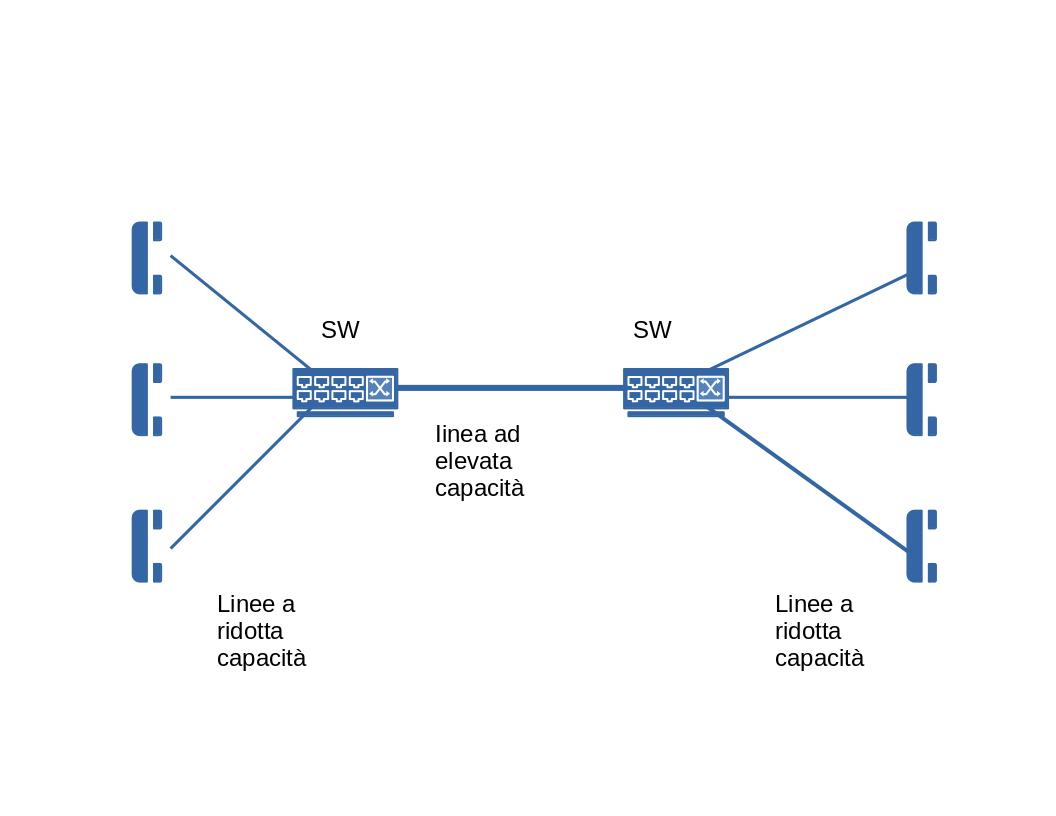
\includegraphics[weight=4cm,height=8cm]{img/Reti a commutazione di circuito.jpg}
  \caption{Reti a commutazione di circuito}
\end{figure}
\subsection{Reti a commutazione di pacchetto}
\begin{itemize}
\item Due dispositivi si scambiano blocchi di dati ({\tt pacchetto})
\item Lo {\it switch} può memorizzare i pacchetti per inviarli successivamente
\item più tipicamente funzione svolta dal {\em router}
\end{itemize}
\begin{figure}[!h]
  \centering
  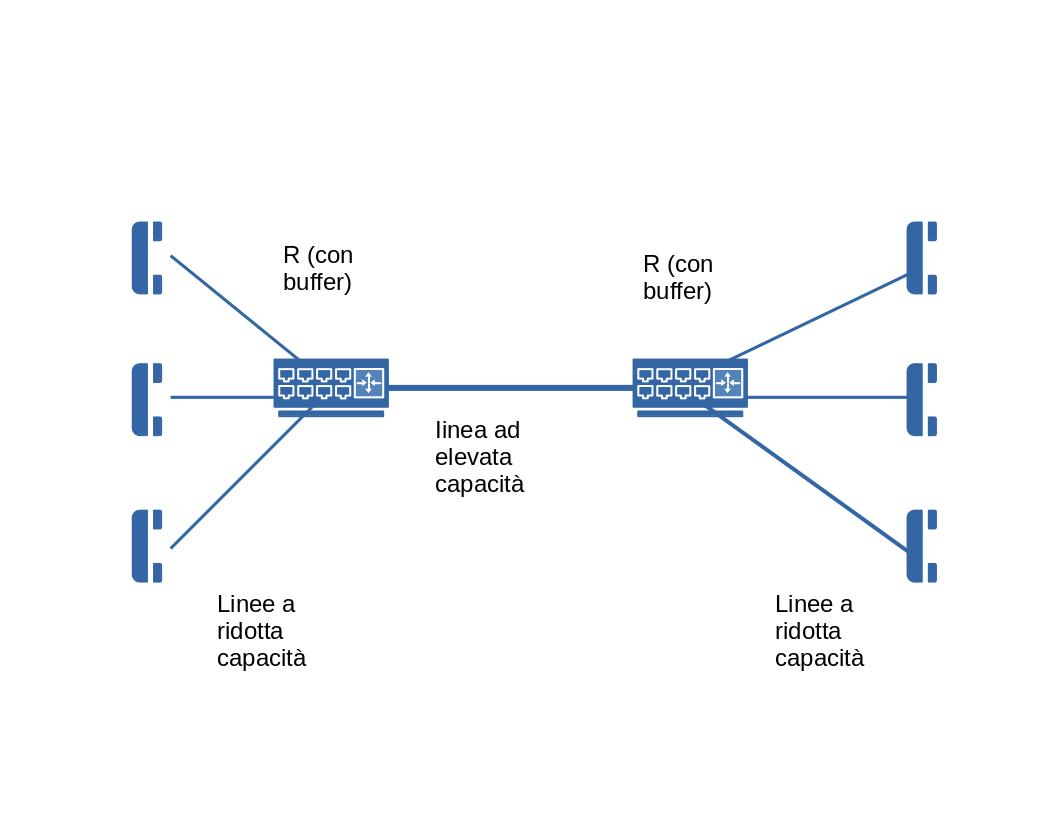
\includegraphics[weight=4cm,height=8cm]{img/Reti a commutazione di pacchetto.jpg}
  \caption{Reti a commutazione di pacchetto}
\end{figure}
\subsection{Implementazioni}
\begin{itemize}
\item Il sistema PDH non è univoco ovunque, me prevede tre standard differenti
  \begin{itemize}
  \item europeo (sistema analogo in india) con base a 32 canali
  \item statunitense con base a 24 canali
  \item giapponese con base a 24 canali
  \end{itemize}
\item Condividono lo stesso meccanismo di base ma differiscono per alcuni dettagli di funzionamento e per le gerarchie di multiplazione
  \begin{itemize}
  \item di fatto assenza di interoperabilità
  \item di fatto poco usati oggigiorno
    \begin{itemize}
    \item sostituiti da sistemi SDH ({\bf che vedremo più avanti in questa lezione})
    \item attivi solo nelle zone terminali delle reti per la multiplazione di traffico telefonico
    \end{itemize}
  \end{itemize}
\end{itemize}
\subsection{Canali telefonici digitali}
\begin{itemize}
\item Modulazione a impulsi codificati
  \begin{itemize}
  \item {\tt Pulse-Code Modulation (PCM)}
  \item anche in altre applicazioni come CD e DVD
  \end{itemize}
\item Campionamento + quantizzazione + rappresentazione binaria (ADC/DAC)
  \begin{itemize}
  \item quantizzazione operazione rumorosa
  \item 8, 16, 20 o 24 bit per campione
  \end{itemize}
\item PCM lineare: i livelli quantizzazione sono linearmente uniformi
\item PCM non lineare
  \begin{itemize}
  \item i segnali maggiormente affetti dell'approssimazione sono quelli a bassa intensità (errore relativo maggiore)
    \item quantizzazione non lineare: livelli più piccoli e ravvicinati nella regione di segnale debole e più distanziati nella regione in cui il segnale è più intenso
  \end{itemize}
\end{itemize}


\chapter{Applicazione delle reti}
\printindex
\end{document}
